\section{Experiments}
\label{sec:experiments}
\subsection{3D Object Detection}
We employed a non-transformer-based architecture for multi-view bird’s eye view (BEV)-based 3D object detection. In this architecture, the multi-view camera images are initially processed by a convolutional image encoder, specifically RegNetY-800MF \cite{RegNet}, with a feature pyramid network based on BiFPN \cite{tan2020efficientdet}. We project the feature levels at /8, /16, and /32 resolutions into the BEV representation using Lift-Splat projection \cite{LSS}. Features from the previous two frames are warped to the current frame using egomotion and then concatenated along the channel dimension, similar to BevDet4D \cite{huang2022bevdet4d}. Gradients produced by the previous frames are not used to update the image encoder. The resulting spatio-temporal BEV features are processed by a ResNet-based \cite{resnet34} BEV backbone. These features are then shared among task-specific heads. We utilize RQR3D \cite{rqr3d} for BEV-based 3D object detection. RQR3D reparametrizes the regression targets for the 3D bounding boxes and implements this reparameterized regression task on an anchor-free single-stage object detector, introducing an objectness head to address class imbalance problems of single-stage object detectors. RQR3D outperforms widely-adopted CenterPoint--based approaches \cite{yin2021center}, yielding lower translation and orientation errors, which are crucial for safe autonomous driving. When using LiDAR, we simply map the point cloud onto the BEV grid and concatenate it with the projected image feature before temporal processing. 


%and bird’s eye view (BEV)-based perception, capitalizing on the framework's ability to transform image-plane features into a spatially structured BEV representation. Specifically, we adopted RegNetY-800MF as the encoder backbone, benefiting from its computational efficiency and strong representational capacity. The encoder outputs feature maps with 256 channels, and a feature pyramid network (FPN) with 256-dimensional channels is constructed to capture multi-scale spatial information. The lifted features are then splatted into the BEV plane, where a decoder with a ResNet-18 backbone processes the BEV features for downstream tasks. For both 2D and 3D object detection, we integrated the Fully Convolutional One-Stage Object Detection (FCOS) framework. In the 2D setting, standard FCOS heads are applied directly on image-plane features to localize objects without anchors. In the BEV space, we employ FCOS BEV-Net heads, which extend FCOS principles to spatially coherent BEV grids, allowing for efficient and anchor-free 3D object detection. This modular design enables consistent prediction across modalities while maintaining high spatial fidelity in the BEV domain.
% The following statistics can be used if needed
% minival 13272 frames on 107 scenes
% val => 47568 frames on 508 scenes
% train => 91847 frames on 1931 scenes

\begin{table}[h]
\caption{The number of object for 3D object detection}
\label{tab:3d_class_counts}
\centering
\begin{tabular}{@{}lccccccc@{}}
\toprule
                  & \textbf{Ambulance} & \textbf{Construction} & \textbf{Crossbike} & \textbf{Walker} & \textbf{Car} & \textbf{Firetruck} & \textbf{Police} \\ \midrule
\textbf{train}    & 2,306               & 50,486                 & 28,980              & 17,247           & 683,332       & 1,070               & 21,181           \\
\textbf{val}      & 2,060               & 2,248                  & 32,177              & 9,703            & 419,697       & 1,495               & 9,803            \\ \bottomrule
\end{tabular}
\end{table}

To align our dataset with the nuScenes \cite{caesar2020nuscenes} benchmark, which provides annotated keyframes at 2 Hz, we downsample our original 10 Hz data to 2 Hz. This conversion ensures consistency in temporal resolution, facilitating fair comparisons and compatibility with existing evaluation protocols. %By matching the frame rate, we maintain uniformity in data representation, which is crucial for accurate benchmarking and analysis in autonomous driving research.
Additionally, we select the scenarios whose name contains keywords such as \textit{accident, construction, dynamic, pedestrian, hazard, emergency,} and \textit{opposite} in order to achieve a more balanced class distribution. The resulting number of objects per category is summarized in Table \ref{tab:3d_class_counts}.
 
We utilize two different sensor configurations: camera-only and camera-LiDAR. Evaluation metrics are adopted from nuScenes \cite{caesar2020nuscenes}, including mean Average Precision (mAP), Average Translation Error (ATE), Average Scale Error (ASE), Average Orientation Error (AOE) and Average Velocity Error (AVE), excluding Average Attribute Error (AAE) as it is not applicable for TaCarla. These metrics provide a comprehensive assessment of detection performance across various object classes. The inclusion of LiDAR modality enhances depth estimation accuracy, leading to improved localization and orientation predictions, as reflected in lower ATE and AOE values. Conversely, the camera-only configuration exhibits higher errors due to the inherent challenges in depth estimation. The detailed class-wise performance metrics are presented in Tables \ref{tab:3d_results_lss} and \ref{tab:3d_results_lss_lidar}, illustrating the comparative effectiveness of both training approaches.


\begin{table}[h]
\caption{Camera-only 3D object detection performance}
\label{tab:3d_results_lss}
\centering
\begin{tabular}{@{}lcccccc@{}}
\toprule
                                  & \textbf{AP} & \textbf{ATE} & \textbf{ASE} & \textbf{AOE} & \textbf{AVE} \\ \midrule
\textbf{Car}                      & 0.459       & 0.444        & 0.147        & 0.012        & 0.559        \\
\textbf{Crossbike}                & 0.324       & 0.242        & 0.094        & 0.057        & 0.165        \\
\textbf{Walker}                   & 0.426       & 0.456        & 0.885        & 1.333        & 0.292        \\
\textbf{Police}                   & 0.381       & 0.249        & 0.056        & 0.011        & 0.048        \\
\textbf{Construction}             & 0.419       & 0.665        & 0.812        & 1.125        & 0.065        \\
\textbf{Ambulance}                & 0.098       & 0.440        & 0.132        & 0.065        & 0.525        \\
\textbf{Firetruck}                & 0.140       & 0.487        & 0.155        & 0.004        & 0.618        \\ \midrule
                                  & mAP: 0.32   & mATE: 0.43   & mASE: 0.33   & mAOE: 0.37   & mAVE: 0.32   \\ \bottomrule
\end{tabular} 
\end{table}

\begin{table}[h]
\caption{Camera-LiDAR 3D object detection performance}
\label{tab:3d_results_lss_lidar}
\centering
\begin{tabular}{@{}lcccccc@{}}
\toprule
                                  & \textbf{AP} & \textbf{ATE} & \textbf{ASE} & \textbf{AOE} & \textbf{AVE} \\ \midrule
\textbf{Car}                      & 0.716       & 0.173        & 0.125        & 0.022        & 0.399        \\
\textbf{Crossbike}                & 0.556       & 0.113        & 0.086        & 0.076        & 0.119        \\
\textbf{Walker}                   & 0.527       & 0.152        & 0.885        & 1.304        & 0.277        \\
\textbf{Police}                   & 0.486       & 0.082        & 0.052        & 0.018        & 0.038        \\
\textbf{Construction}             & 0.657       & 0.253        & 0.821        & 1.125        & 0.098        \\
\textbf{Ambulance}                & 0.428       & 0.254        & 0.100        & 0.074        & 0.283        \\
\textbf{Firetruck}                & 0.452       & 0.270        & 0.108        & 0.002        & 0.344        \\ \midrule
                                  & mAP: 0.55   & mATE: 0.19   & mASE: 0.31   & mAOE: 0.37   & mAVE: 0.22   \\ \bottomrule
\end{tabular} 
\end{table}



\subsection{Lane Detection}
\begin{table}[t]
  \caption{Centerline and Lane Divider Detection Results of TopoBDA architecture for TaCarla Dataset.}
  \label{tab: topobda_tacarla}
  \centering
  \begin{tabular}{lccc}
    \toprule
    \textbf{Detection Task} & \textbf{\( \text{AP}_f \)} & \textbf{\( \text{AP}_c \)} & \textbf{F1\(_{1.5}\)} \\
    \midrule
    Centerline Detection & 58.2 & 60.9 & 73.8 \\
    Lane Divider Detection & N/A & 60.2 & 75.6 \\
    \bottomrule
  \end{tabular}
\end{table}

Lane detection consists of two sub-tasks which are lane divider detection and centerline detection. For the lane divider and centerline detection tasks, Chamfer Distance-based Average Precision (\( \text{AP}_c \)) \cite{li2022hdmapnet, liao2024maptrv2} and Frechet Distance-based Average Precision (\( \text{AP}_f \)) \cite{wang2024openlane, li2023graph, wu2023topomlp} metrics were utilized. These metrics are commonly used in the literature to evaluate the geometric similarity between predicted and ground-truth polylines. For \( \text{AP}_f \), the thresholds are 1, 2, and 3 meters, and for \( \text{AP}_c \), the thresholds are 0.5, 1, and 1.5 meters. Additionally, the F1 metric is included, which is another widely used metric in the literature for assessing lane detection performance \cite{Guo_2020, chen2022persformer}. In F1 metric calculation, if 75\% of the points are within the predetermined threshold, the instances are assumed to be true positives. In this study, this threshold is set to 1.5 meters, in accordance with the literature. For all evaluation metrics, 11 ground truth points are utilized.

For the training of both centerlines and lane dividers, the TopoBDA study \cite{kalfaoglu2024topobda} was utilized, which incorporates specialized attention structures and advanced polyline training practices derived from the TopoMaskV2 study \cite{kalfaoglu2024topomaskv2}. The Bezier Deformable Attention mechanism, a key innovation of TopoBDA, focuses attention around Bezier keypoints rather than a single central point. This approach enhances the efficiency of polyline learning by improving the detection and representation of elongated and thin polyline structures. 

% \begin{figure}[t]
%   \centering
%   \includegraphics[width=1.0\linewidth]{figures/pv_topobda.pdf}
%   \caption{Perspective View (PV) results demonstrating the performance of TopoBDA on the TaCarla dataset using a six-camera setup. GT denotes the ground truth, and Pred denotes the predictions.}
%   \label{fig: pv_samples}
% \end{figure}

\begin{figure}[t]
  \centering
  \includegraphics[width=1.0\linewidth]{figures/bev_tacarla.pdf}
  \caption{Bird's Eye View (BEV) results demonstrating the performance of TopoBDA on the TaCarla dataset. GT denotes the ground truth, and Pred denotes the predictions. GT + Pred shows the overlaid results of both, facilitating visual assessment of localization performance.}
  \label{fig: bev_samples}
\end{figure}

The results for the training of TopoBDA for lane divider and centerline detection are presented in Table \ref{tab: topobda_tacarla}. The experimental details for this training are consistent with those outlined in the TopoBDA study \cite{kalfaoglu2024topobda} except that the training duration is set to 6 epochs. The Frechet Distance-based Average Precision (\( \text{AP}_f \)) is marked as N/A because the Frechet distance emphasizes directional information, which is not relevant to the lane divider detection task. In the experiments, the TaCarla dataset is utilized in a 2Hz configuration and the validation set is subsampled further with a factor of 5. 

Bird's Eye View (BEV) demonstrations are presented in Figure \ref{fig: bev_samples}, respectively. These figures include visualizations of both centerlines and lane dividers. In the figure, GT denotes the ground truth, while Pred represents the predictions made by TopoBDA. Additionally, Figure \ref{fig: bev_samples} includes an overlaid visualization (GT + Pred), which aids in understanding the localization performance. It is noteworthy that in junction regions, lane dividers are excluded, whereas centerlines are included, as illustrated in Figure \ref{fig: bev_samples}.


\begin{figure}[h]
  \centering
  \includegraphics[width=6cm]{figures/tl_red.jpg} 
  \includegraphics[width=6cm]{figures/tl_green.jpg}
  \caption{Outputs of the FCOS traffic light model}
\end{figure}

\subsection{Traffic Light Detection}
The dataset we propose consists of 238,780 and 187,987 images containing traffic light instances in the training and validation sets, respectively. Every individual image in the dataset consists of a single traffic light instance with three distinct classes; \textit{red}, \textit{yellow}, \textit{green}. Every instance is labeled with their 2D bounding box and corresponding class. For the traffic light detection task, we employed off the shelf single-stage object detector FCOS \cite{fcos} with ResNet-50 backbone as a baseline. We use 1x training schedule; we train for 12 epochs with a learning rate of $1e^{-3}$. We schedule the learning rate at 8th and 11th epochs with a rate of $0.1$. We report COCO style \cite{COCO} $\mathrm{AP}$ and $\mathrm{AP_{50}}$ in Table \ref{tab:TLR}.

\begin{table}[th]
  \caption{Traffic Light Detection task results in TaCarla.}
  \label{tab:TLR}
  \centering
  \begin{tabular}{lcc}
    \toprule
    \textbf{Model} & $\mathrm{AP}$ & $\mathrm{AP_{50}}$ \\
    \midrule
    FCOS \cite{fcos} & $59.5$ & $88.2$ \\
    \bottomrule
  \end{tabular}
\end{table}



\subsection{Planning}

\begin{figure}[h]
  \centering
  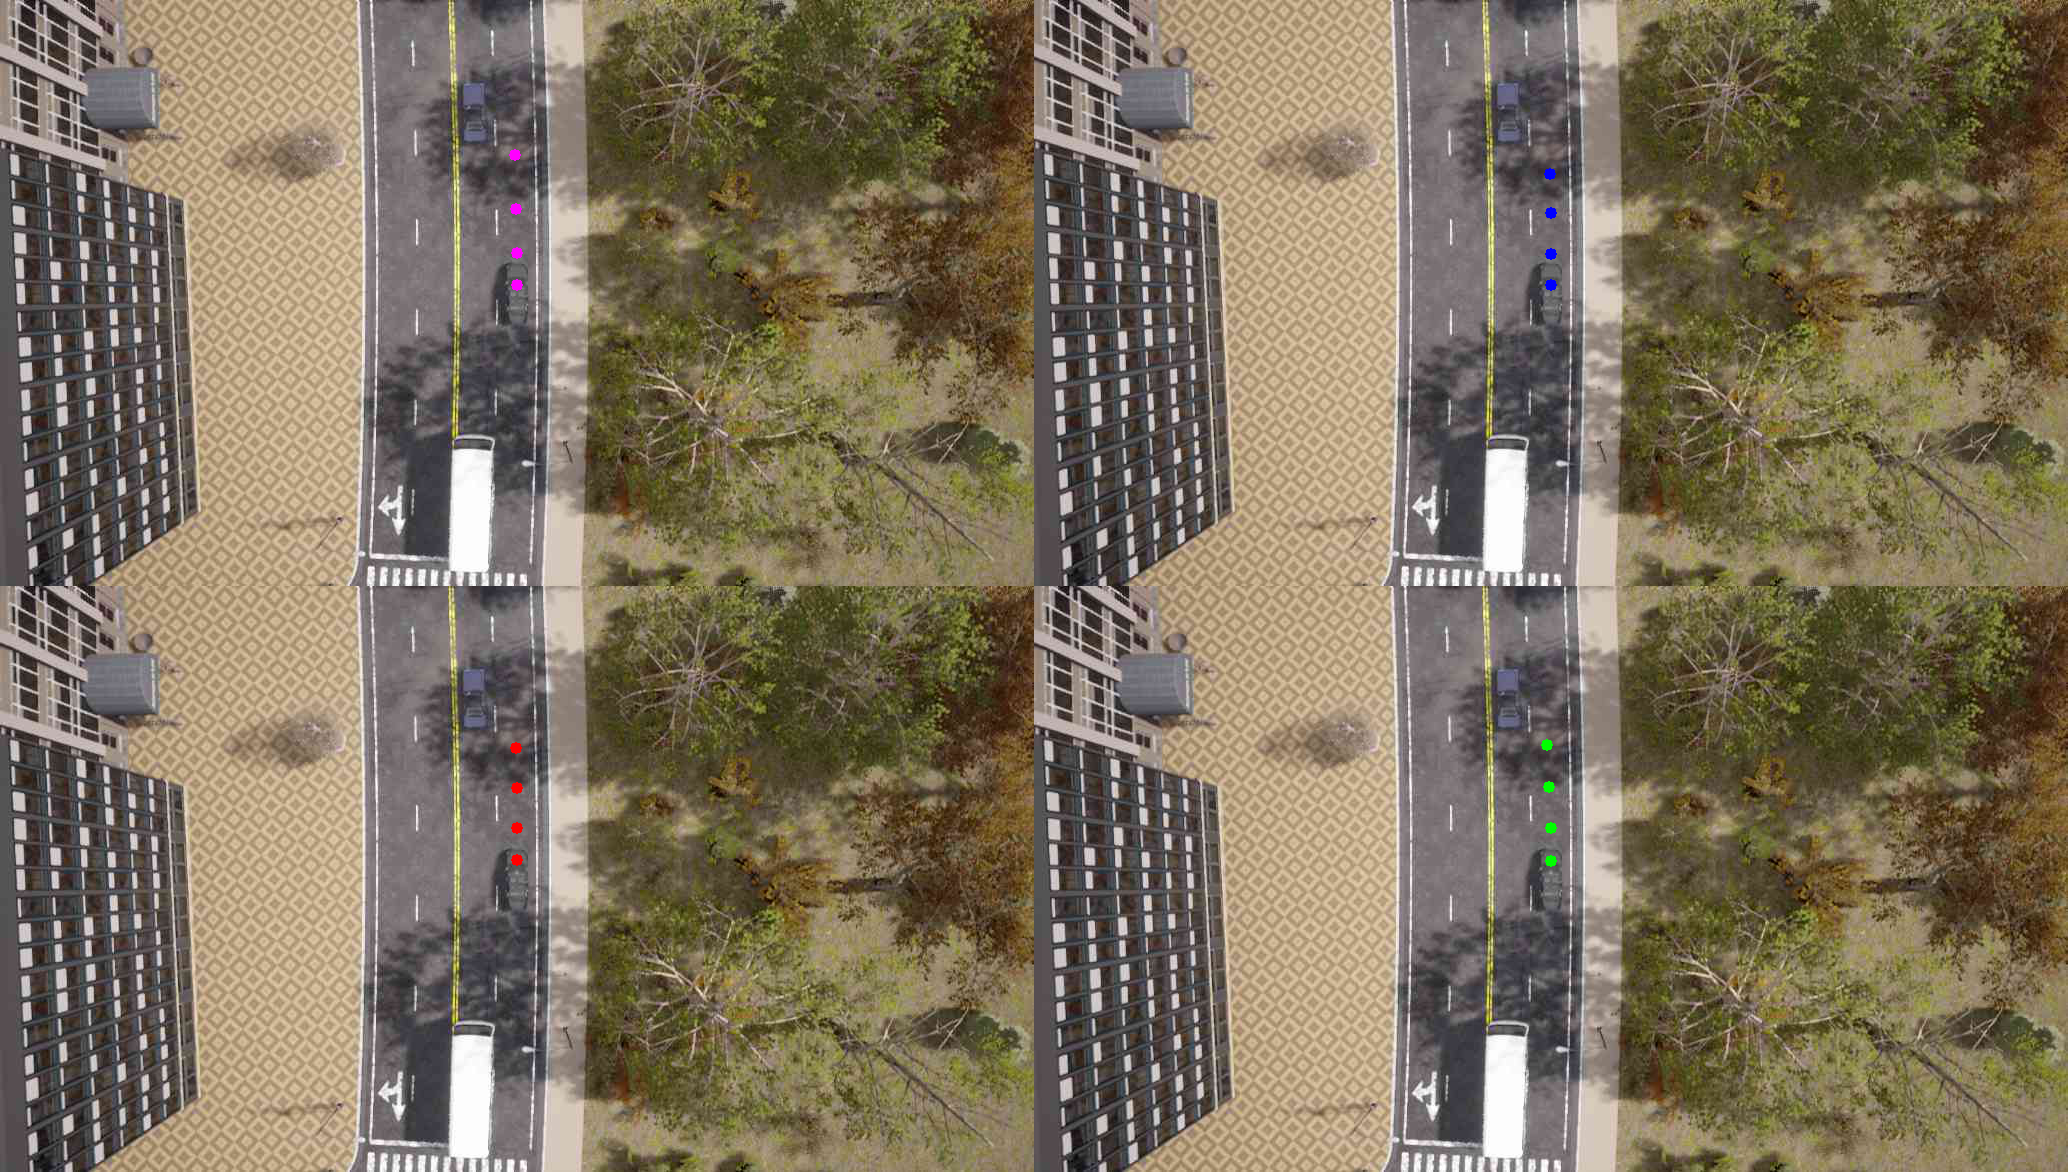
\includegraphics[width=10cm]{figures/planning.png} 
  \caption{Waypoints from ground truth(Top Left), PlanT(Top Right), Transfuser(Bottom Left), and DiffusionDrive (Bottom Right) models.}
\end{figure}

For the planning task, we trained three baseline agents: Transfuser~\cite{transfuser}, DiffusionDrive~\cite{diffusiondrive}, and PlanT~\cite{planT}. 
We choose Transfuser and DiffusionDrive upon their great success in Navsim~\cite{navsim} dataset. Both agents trained with the same Resnet-34 backbone~\cite{resnet34} which uses 3 forward facing cameras and LiDAR. The cameras are cropped and concatenated as a single image of size $256x1024$ and LiDAR point clouds rasterized with a BEV size $256x256$. Both agents use the same ego status input which consists of vectorel velocity, acceleration and driving command. The driving command is calculated as it is in Navsim~\cite{navsim}. We used our annotated lane guidance waypoints by classifying the point 15m away from ego position as left, right or straight by checking the lateral distance with a threshold of 2m. We trained DiffusionDrive for 6 epochs  and Transfuser for 3 epochs with a learning rate of $7.5 \times 10^{-5}$ on 8 NVIDIA A100 GPUs with a total batch size 64. We filtered our training set scenarios with driving score >70. During training, we sampled ground truth trajectories with 2Hz which gives 8 waypoints for a 4 seconds horizon. The implementation acrhitecture is the same with DiffusionDrive paper~\cite{diffusiondrive} where we used 20 anchors clustered from our dataset. During evaluation we used 2 denoising steps as the authors use in Navsim challenge~\cite{navsim}. 

% EXPLAIN PLANT HERE
The other chosen planning model was the PlanT model \cite{planT} because it is one of the best planning models that utilizes ground truth information. Therefore, by training the PlanT model, we can verify our labels in the dataset. We trained the PlanT model for 50 epochs, with a batch size of 16 and a learning rate of  $10^{-4}$.

%Another reason is that, although Transfuser is more popular in the literature due to its simplicity and strong performance, the PlanT model \cite{planT} outperforms Transfuser when used with a perception model in this study \cite{planT}.

For the evaluation of the trained agents, we provide both open-loop and closed-loop results. Open-loop results are calculated by computing the average displacement error (ADE), the final displacement error (FDE), the average head error (AHE) and the final head error (FHE) between the predicted and ground-truth trajectories as it is calculated in NuPlan~\cite{nuplan}. We provide our metrics for 3 different prediction horizons in seconds with 2Hz sampling rate. We used the Town13 validation set of our dataset where episodes are limited to 400 frames since the complex scenarios are triggered at the beginning of the episodes. See Table~\ref{tab:openloop-results} for the results. For the closed-loop evaluation, we simplified our validation dataset routes to 36 scenarios and run them with CARLA Leaderboard V2~\cite{CARLA} framework. We provide scenario-specific open-loop and closed-loop results in Appendix. 

\begin{table}[h]
  \caption{Open-loop results on validation set with 1s, 2s and 4s planning horizons ($\mathcal{H}$).}
  \label{tab:openloop-results}
  \centering
  \setlength{\tabcolsep}{4pt}
  \renewcommand{\arraystretch}{1.2}
  \begin{tabular}{lccccc|c|cccc}
    \toprule
    \multirow{2}{*}{Model} & \multicolumn{5}{c|}{Input} & \multirow{2}{*}{$\mathcal{H}$} & \multicolumn{4}{c}{Results} \\
    \cmidrule(lr){2-6} \cmidrule(lr){8-11}
    & Camera & LiDAR & GT Box & Ego Status & & & ADE & FDE & AHE & FHE \\
    \midrule
    \multirow{3}{*}{DiffusionDrive \cite{diffusiondrive}} 
      &           &           &            &           & &$4$&$2.69$& $5.58$ & $0.27$ & $0.21$ \\
      & \checkmark & \checkmark &  & \checkmark        & & $2$&$1.14$ & $2.14$ & $0.21$ & $0.21$ \\
      &           &           &            &           & & $1$ & $0.51$ & $0.78$ & $0.12$ & $0.12$ \\
    \midrule
    \multirow{3}{*}{PlanT \cite{planT}} 
      &           &           &            &           & & $4$ & $-$ & $-$ & $-$ & $-$ \\
      &           &           & \checkmark &           & & $2$ & $1.03$ & $1.71$ & $0.36$ & $0.34$ \\
      &           &           &            &           & & $1$ & $-$ & $-$ & $-$ & $-$ \\
    \midrule
    \multirow{3}{*}{Transfuser \cite{transfuser}} 
      &           &           &            &           & & $4$ & $2.29$ & $4.97$ & $0.23$ & $0.27$ \\
      & \checkmark & \checkmark &  & \checkmark        & & $2$ & $0.91$ & $1.74$ & $0.23$ & $0.27$ \\
      &           &           &            &           & & $1$ & $0.40$ & $0.59$ & $0.22$ & $0.22$ \\
    \bottomrule
  \end{tabular}
\end{table}

%\subsection{Prediction}
%For the other vehicle's future prediction task, the Fiery \cite{hu2021fieryfutureinstanceprediction} model was utilized. Fiery has shown exceptional performance on well-established benchmark datasets like NuScenes \cite{caesar2020nuscenes} and Lyft \cite{li2023largecarfollowingdatabased}, surpassing earlier prediction models in metrics such as Intersection-over-Union (IoU) and Video Panoptic Quality (VPQ). This highlights its ability to effectively predict future events in realistic driving environments. The Fiery model was trained using the original hyperparameters: 20 epochs, a batch size of 12, and a learning rate of 3×$10^{-3}$.
